Programinės įrangos kūrimas pirmiausiai pradedamas nuo užduoties analizės.
Užduotis yra sukurti programinę įranga, kuri gali dirbti su \textit{STM32F411} platforma ir bendrauti su \textit{MPU 9250} jutikliu.

\begin{figure}[H]
    \centering
    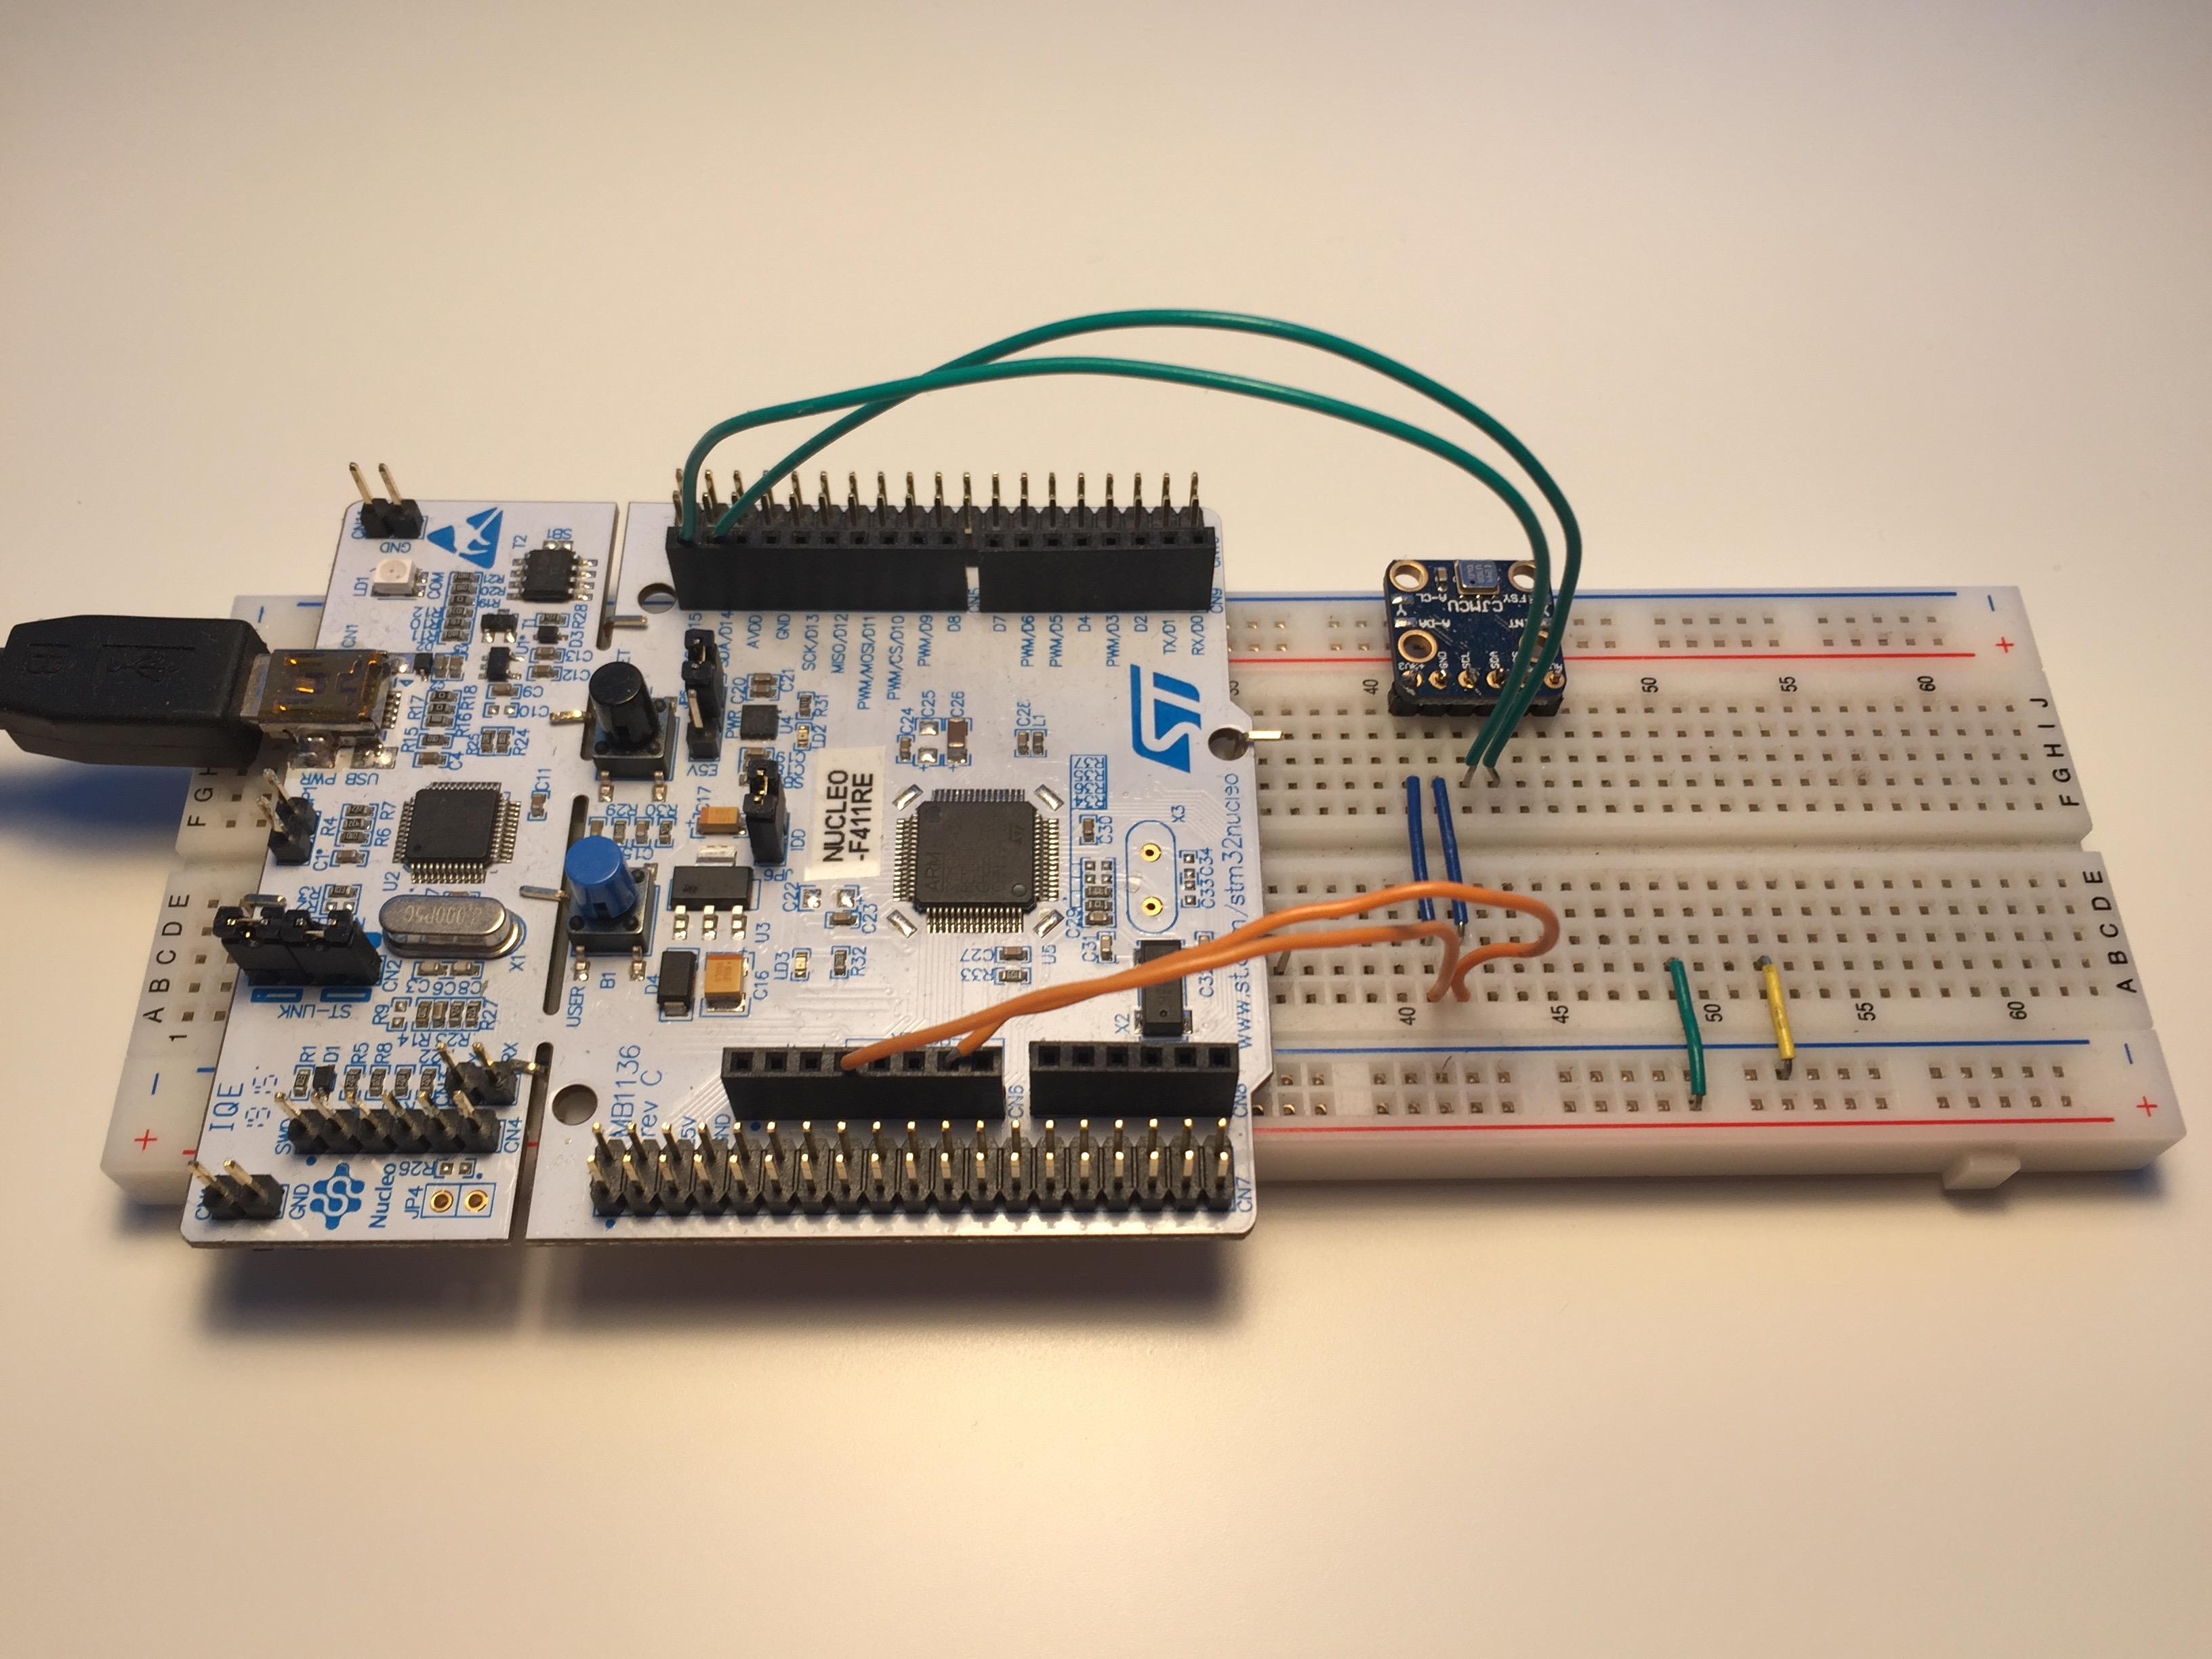
\includegraphics[width=300px]{img/naudojama-platforma.jpg}
    \caption{Naudojama STM32 platforma.}
    \label{fig:web-idea}
\end{figure}

ARM šeimos naudojama platforma suteikia pakankamai galingus įrankius darbo su sistema. Pats paprasčiausias ir priimtiniausias įrankis jokios patirties įterptinėse sistemose neturinčiam programuotojui yra tiesiogiai tinklapyje veikiantis redaktorius, kuris sugeba pasirūpinti reikiamomis bibliotekomis, bei sukompiliuoti visą reikiamą kodą į vieną binarinę bylą, kurią galima tiesiog perkelti į USB sąsaja prijungta plokšte. \textit{STM32F411} platformoje įmontuotas programuotojas automatiškai perrašo procesoriaus vykdomą programinį kodą ir paleidžia programą.

\begin{figure}[H]
    \centering
    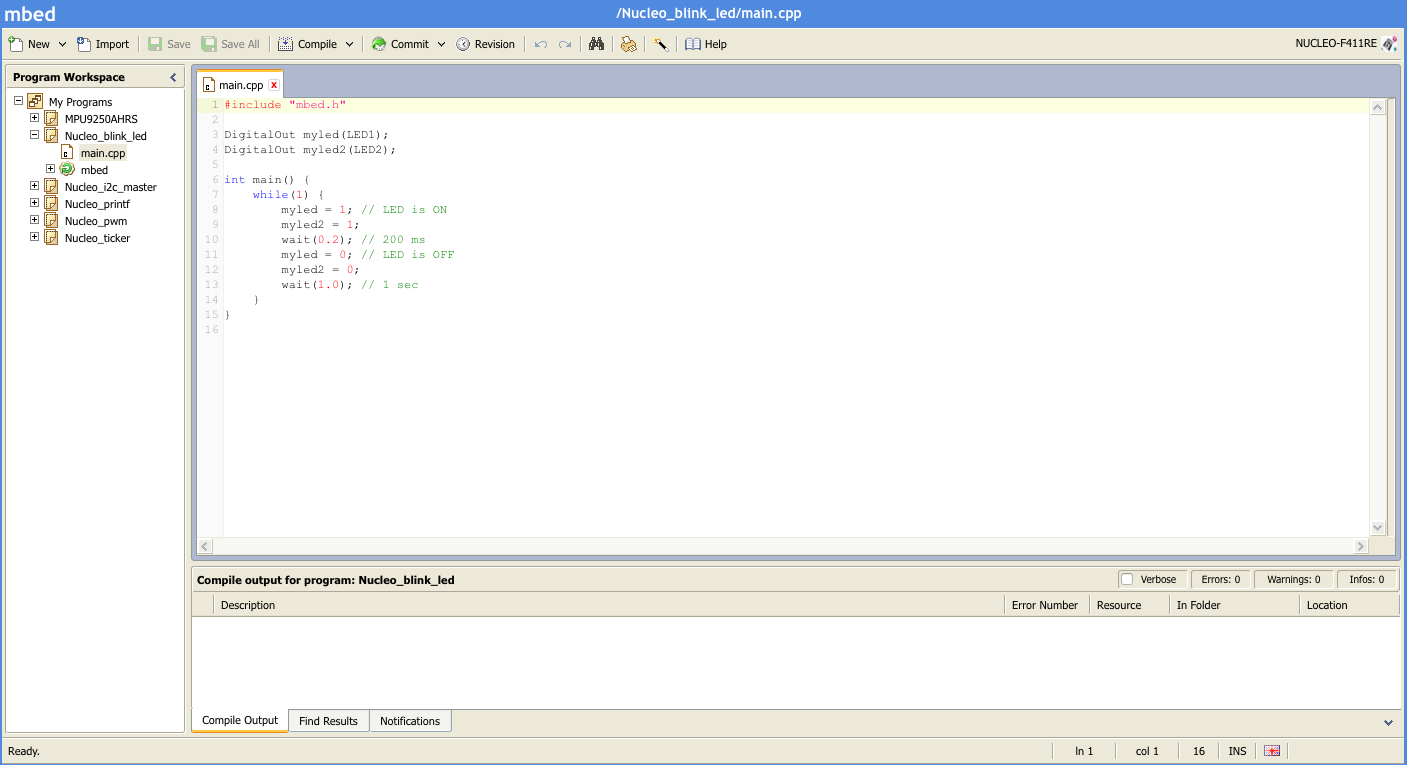
\includegraphics[width=300px]{img/web-idea.png}
    \caption{Per paprastą tinklapį pasiekiama įterptinės sistemos programinės įrangos vystymo sąsaja \cite{mbedC9:online}.}
    \label{fig:web-idea}
\end{figure}

Tačiau toks programinės įrangos vystymas gali būti labai lėtas ir sugeneruoti labai daug parsiuntimo bylų skaičių. 
Dėl šios priežasties perkeliam visą programinės įrangos bibliotekas ir kompiliavimą į lokalią mašiną.
Ta pati internetinė platforma leidžia eksportuoti esamą projektą į GNU Toolchain aplinkos projektą, kartu paruošia ir tvarkingą \textit{Makefile}, kurį pačiam rašyti yra labai problematišką.

Pats kompiliavimas vykdomas labai paprastai dėl gražaus \textit{Makefile}, kuris yra sugeneruotos ankščiau aprašytos platformos. Viso labo ką reikia padaryti, tai paleisti \textit{make} komandą terminale ir bus pateikiama bin bylą, kurią toliau reikia įrašyti į įterptinę įrangą. 

Rašymas į įterptinę sistemą vykdomas taip pat konsolės pagalba, naudojant \textit{stlink} programinį paketą. Rašymo komanda \textit{st-flash} pradžioje priima operacijos komanda, kuri rašymo atveju yra \textit{write}, toliau seka objekto byla, kuria norime įrašyti į įterptinę sistemą, \textit{main.bin}, bei galutinis argumentas yra pradžios adresas, \textit{0x8000000}. Visa komanda ir galimas programos išvedimo rezultatas yra pateikiamas \ref{fig:st-link-write} pavyzdyje.

\begin{figure}[H]
    \centering
    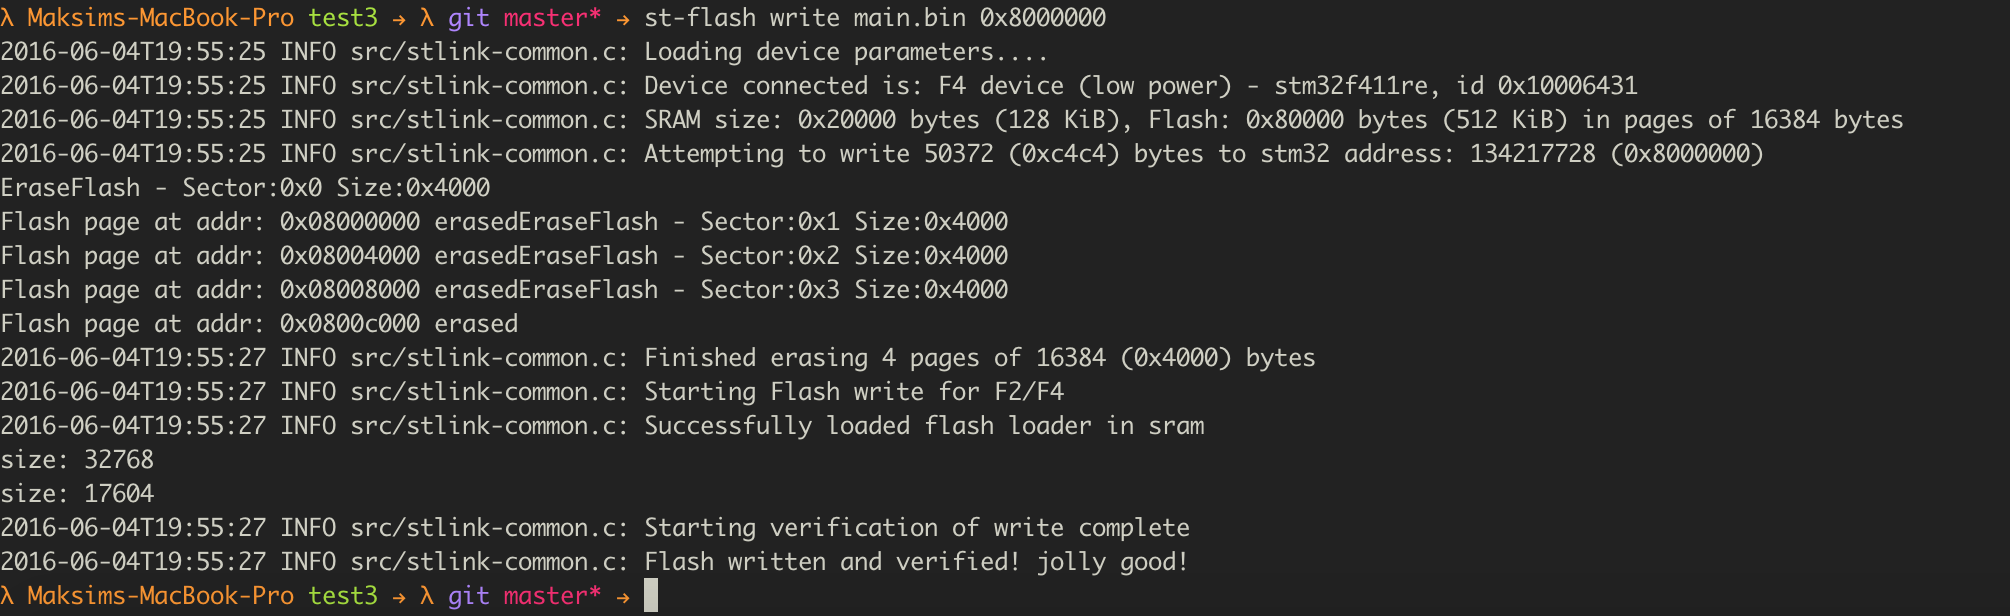
\includegraphics[width=500px]{img/st-link-write.png}
    \caption{Programinio patekto \textit{stlink} bin bylos rašymas į įterptinę sistemą.}
    \label{fig:st-link-write}
\end{figure}

Pagaminta programinė įranga yra pateikiama atvirai prieigai, pritaikant BSD licenciją.

\begin{quote}
    https://github.com/dummas/upgraded-giggle
\end{quote}
